\chapter{Biểu diễn và kiến trúc bốn phương pháp}
\label{chap:model}
Chương~\ref{chap:related} xác định ba hướng biểu diễn được lựa chọn. Chương này mô tả đúng các cấu hình thực thi: TF--IDF với SVM/LR, LSTM hai chiều với embedding học từ đầu và PhoBERT-base-v2 có tiền huấn luyện. Các khác biệt về stopword, tiêu đề và đơn vị cắt được công khai để diễn giải kết quả so sánh.
\section{TF--IDF và hai bộ phân loại tuyến tính}
\label{sec:linear_models}
SVM và Logistic Regression dùng cùng cách tạo đặc trưng từ corpus chuẩn hóa. Sau khi chốt corpus và phép chia, tiêu đề đã phân đoạn được lặp thêm hai lần trước chuỗi tiêu đề--nội dung, tạo ba lần xuất hiện của tiêu đề. Hai notebook dùng danh sách stopword riêng nhưng có cùng nội dung, gồm 1.959 mục sau chuẩn hóa; hash bắt đầu \texttt{8560838c}. Stopword được loại ở bước biểu diễn cho mô hình, không dùng để xác định nhóm trùng của corpus chung.

\subsection{Từ tần suất đến vector thưa}
Với thuật ngữ $j$ và tài liệu $d$, biểu diễn dùng TF logarit, IDF có làm trơn và chuẩn hóa $L_2$:
\begin{align}
\operatorname{tf}_{d,j}&=1+\log n_{d,j}\quad(n_{d,j}>0),\\
\operatorname{idf}_j&=\log\frac{1+N_{train}}{1+\operatorname{df}_j}+1,\\
v_d&=\frac{\operatorname{tf}_d\odot\operatorname{idf}}{\|\operatorname{tf}_d\odot\operatorname{idf}\|_2}.
\end{align}
Từ vựng và IDF chỉ fit trên 139.975 mẫu train. Validation và test đi qua transform với các tham số đã cố định. Cấu hình được chọn giữ unigram và bigram, tối đa 150.000 đặc trưng, \texttt{min\_df=3}, \texttt{max\_df=0.98}; số chiều thực tế là 150.000. Không có SVD trong pipeline này. Các vector được lưu và tính toán dưới dạng thưa, không tạo ma trận dense toàn corpus.

Việc lặp tiêu đề tăng tần suất tín hiệu đầu bài, nhưng hệ số ba không có nghĩa giá trị TF--IDF cuối tăng đúng ba lần: TF logarit và chuẩn hóa $L_2$ còn biến đổi tỷ lệ. Bigram được tạo trên chuỗi ghép, nên cũng có thể xuất hiện ở ranh giới các lần lặp tiêu đề. Toàn văn không bị cắt theo số vị trí như mô hình neural, song thứ tự xa và cấu trúc lập luận không được giữ trong một vector TF--IDF \citep{kowsari2019}.

\subsection{SVM tuyến tính và Logistic Regression}
\texttt{LinearSVC} dùng regularization $L_2$, squared hinge loss và cơ chế một-chống-phần-còn-lại cho 20 lớp. Trong bộ phân loại lớp $c$, nhãn nhị phân $y_{i,c}\in\{-1,+1\}$ tạo hạng mất mát
\begin{equation}
\ell_{i,c}=\bigl[\max(0,1-y_{i,c}(w_c^\top v_i+b_c))\bigr]^2.
\end{equation}
Hệ số $C$ điều khiển đánh đổi regularization và mất mát. Điểm $s_c=w_c^\top v+b_c$ là margin, chưa phải xác suất; nhãn được chọn bằng argmax của 20 điểm. SVM trong thực nghiệm là tuyến tính, khác kernel RBF của một số nghiên cứu ở chương~\ref{chap:related}.

Logistic Regression dùng solver L-BFGS cho phân loại multinomial với regularization $L_2$. Logits tuyến tính được chuẩn hóa thành xác suất lớp:
\begin{equation}
p_c(v)=\frac{\exp(w_c^\top v+b_c)}{\sum_{j=1}^{20}\exp(w_j^\top v+b_j)}.
\end{equation}
Mục tiêu là log-loss có trọng số lớp, khác squared hinge của SVM. Cả hai có cùng thông tin từ vựng, nhưng nghiệm tối ưu và thang điểm khác nhau. Xác suất do LR học vẫn cần kiểm tra calibration; tối ưu log-loss không bảo đảm confidence đúng trên mọi nhóm bài.

\begin{table}[htbp]\centering\small\caption{Hai cấu hình tuyến tính được chọn bằng validation.}\label{tab:linear_config}
\begin{tabular}{lcc}\toprule Thuộc tính & SVM & Logistic Regression\\\midrule
Đặc trưng & \multicolumn{2}{c}{TF--IDF unigram/bigram, 150.000 chiều}\\
Trọng số lớp & balanced & balanced\\
$C$ & 0,5 & 3,0\\
Solver & liblinear, dual auto & L-BFGS\\
Ngưỡng hội tụ & $10^{-4}$ & $10^{-4}$\\
Số vòng tối ưu & 119 & 138\\
Giới hạn vòng & 5.000 & 500\\
Luồng CPU & 4 & 4\\\bottomrule
\end{tabular}\end{table}

\subsection{Đặc trưng học được và giới hạn diễn giải}
Hệ số dương lớn cho biết đặc trưng tăng điểm của lớp trong mô hình đã fit. Với Nông thôn mới, SVM có hệ số 3,1823 cho \texttt{nông\_thôn}; LR có hệ số 13,5690 cho cùng đặc trưng và 6,1810 cho bigram \texttt{xây\_dựng nông\_thôn}. Không so độ lớn giữa hai model như một thang quan trọng chung: mục tiêu, $C$ và thang score khác nhau. Hệ số cũng không phải tác động nhân quả hoặc một lời giải thích đầy đủ cho từng bài.

\begin{figure}[tbp]\centering
\begin{subfigure}[t]{.85\textwidth}\centering
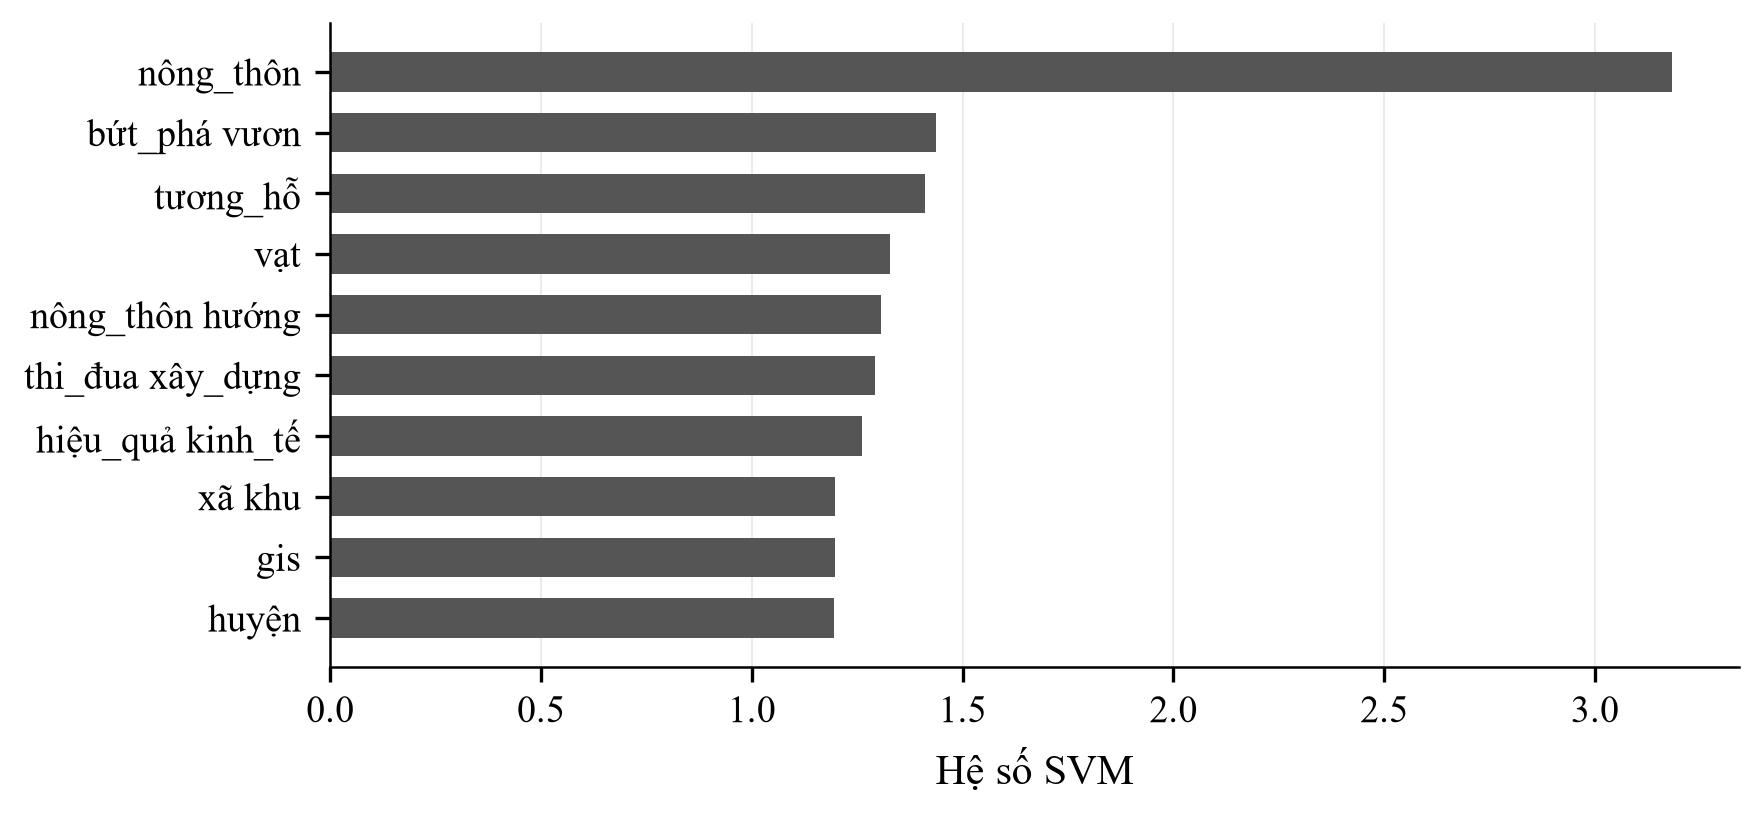
\includegraphics[width=\linewidth]{assets/compact/svm_features.png}\caption{Linear SVM.}\end{subfigure}\par\medskip
\begin{subfigure}[t]{.85\textwidth}\centering
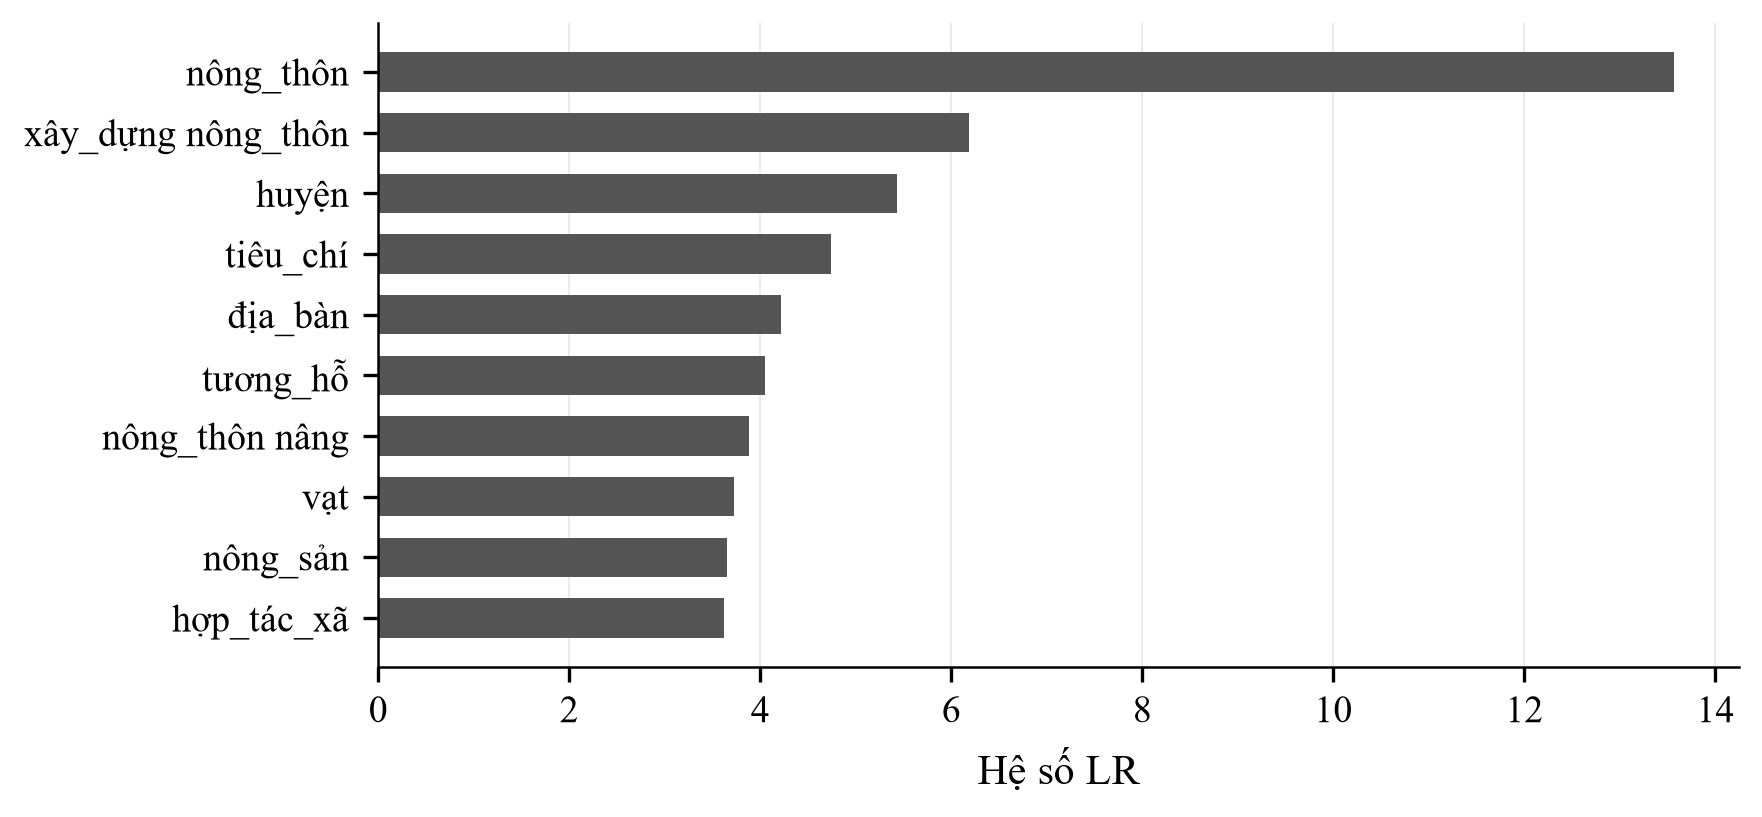
\includegraphics[width=\linewidth]{assets/compact/lr_features.png}\caption{Logistic Regression.}\end{subfigure}
\caption{Đặc trưng có hệ số dương lớn ở Nông thôn mới; thang hệ số không trực tiếp tương đương giữa hai model.}\label{fig:linear-features}\end{figure}

Việc bỏ stopword giảm một phần vốn từ thường xuất hiện, nhưng cũng có thể bỏ tín hiệu diễn ngôn hoặc cách viết của tòa soạn. N-gram còn khai thác cụm cục bộ sau bước lọc, với từ nhiều âm tiết đã được nối bằng PyVi. Vì thế, một bigram là hai đơn vị phân đoạn, không nhất thiết hai âm tiết cách trắng ban đầu. Vocabulary train cố định cũng có thể bỏ thuật ngữ mới ở test; khác biệt này không đồng nhất với UNK của model chuỗi.

Một hệ số lớn không có nghĩa mọi bài chứa term đó phải nhận nhãn tương ứng. Điểm tuyến tính còn cộng các đặc trưng khác và bias, trong khi giá trị term đã qua IDF cùng chuẩn hóa vector. Bỏ một term khỏi một bài có thể thay chuẩn hóa và làm đổi cả vector. Phân tích hệ số cung cấp tín hiệu toàn cục của model được fit, chưa là phép giải thích cục bộ có kiểm soát cho một dự đoán cụ thể.
\FloatBarrier

\section{Biểu diễn chuỗi và kiến trúc BiLSTM}
\label{sec:bilstm}
Phương pháp LSTM trong thiết kế được thực thi bằng biến thể hai chiều BiLSTM. Embedding được khởi tạo và học từ train, không nạp Word2Vec, PhoW2Vec hay encoder tiền huấn luyện. Chuỗi đầu vào giữ stopword và chỉ ghép tiêu đề một lần với nội dung. Vì vậy, đây là một đối chứng học biểu diễn tuần tự có giám sát, khác cả TF--IDF và PhoBERT có pretraining.

\subsection{Vocabulary, từ ngoài từ vựng và Head--Tail}
Vocabulary đếm từ trên train, lấy từ có tần suất ít nhất hai, sắp theo tần suất giảm rồi theo từ điển khi bằng nhau. Tổng 50.000 ID gồm PAD bằng 0, UNK bằng 1 và 49.998 từ. Token ngoài vocabulary được đưa về UNK; embedding PAD không được cập nhật như từ nội dung. Không học vocabulary từ validation/test để giảm tỷ lệ từ lạ một cách không hợp lệ.

Cấu hình được chọn giới hạn 512 \emph{từ đã phân đoạn}. Bài dài giữ 256 từ đầu và 256 từ cuối, không thêm BOS/EOS. Bài ngắn được giữ đầy đủ; mỗi batch pad đến độ dài lớn nhất của các mẫu trong batch, rồi dùng packed sequence để bỏ padding khỏi quá trình recurrent. Head--Tail vẫn bỏ phần giữa và nối hai đoạn không kề nhau, nhưng đơn vị cắt khác 254 subword nội dung của PhoBERT.

Trên corpus 199.965 bài, 44,14\% vượt 512 từ; tỷ lệ từ giữ trung bình là 87,13\%. Hai giá trị được tính từ độ dài đã xuất, không phải một lần tokenize mới. Tỷ lệ OOV trên toàn chuỗi train/validation/test lần lượt là 0,7782\%, 0,8714\% và 0,8696\%. Audit OOV tính trước cắt Head--Tail; không đồng nhất với tỷ lệ UNK trong tensor cuối hoặc lượng thông tin ngữ nghĩa bị mất.


Việc đặt UNK chỉ xử lý khả năng tra ID, không bổ sung nghĩa riêng cho mỗi từ lạ. Những từ ngoài vocabulary khác nhau cùng đi vào một embedding UNK; chúng vẫn có thể được phân biệt một phần bởi các từ bao quanh, nhưng thông tin từ vựng gốc đã mất. Tỷ lệ OOV thấp trên snapshot chưa dự báo tỷ lệ ở tin tương lai chứa tên riêng và thuật ngữ mới.

Packed sequence giúp trạng thái kết thúc phản ánh độ dài thật của bài, tránh recurrent tiếp tục quét nhiều PAD tới độ dài batch. Hai hướng đều quét chuỗi sau Head--Tail; hướng ngược không khôi phục phần giữa đã bị bỏ. Khi nối hai đoạn xa nhau, mô hình vẫn coi chúng là một chuỗi kề nhau, một giả định chung của cách cắt này với PhoBERT.



\subsection{Cơ chế cổng và trạng thái chuỗi}
LSTM duy trì hidden state $h_t$ cùng cell state $c_t$. Forget gate quyết định phần trạng thái cũ giữ lại, input gate điều chỉnh phần thông tin mới ghi vào, output gate điều chỉnh thông tin đưa ra hidden. Dạng cập nhật chuẩn giải thích vai trò của các cổng trong recurrent layer được dùng:
\begin{equation}c_t=f_t\odot c_{t-1}+i_t\odot\widetilde c_t,\qquad h_t=o_t\odot\tanh(c_t).\end{equation}
Các vector gate có giá trị sigmoid và được học từ embedding hiện tại cùng hidden trước đó; candidate cell dùng biến đổi phi tuyến. Đây là trạng thái theo chuỗi, không phải một đặc trưng TF--IDF được coi tùy ý như trục thời gian. Cổng cho phép điều chỉnh truyền thông tin nhưng không bảo đảm nhớ đủ mọi chi tiết qua một bài dài \citep{kowsari2019}.

Hai hướng của BiLSTM có tham số riêng và quét theo hai thứ tự ngược nhau. Chúng cung cấp hai cách tổng hợp cùng chuỗi đã giữ, rồi head nhận vector nối; số lớp recurrent vẫn là một, không biến thành mạng nhiều tầng vì có hai hướng. Dropout bên ngoài recurrent có vai trò regularization, không bổ sung token hoặc tri thức ngôn ngữ tiền huấn luyện.


\subsection{Trạng thái hai chiều và đầu phân loại}
Embedding có chiều 200; một recurrent layer có hidden size 128 cho mỗi hướng. Các cổng forget, input và output lần lượt điều chỉnh thông tin cũ giữ lại, thông tin mới ghi vào cell state và phần trạng thái được xuất theo chuỗi \citep{kowsari2019}. Mô hình quét chuỗi đã cắt ở cả hai hướng, rồi ghép trạng thái kết thúc phép quét xuôi và ngược:
\begin{equation}
r=[\overrightarrow h_{\mathrm{end}};\overleftarrow h_{\mathrm{end}}]\in\mathbb R^{256},\qquad
z=W\operatorname{Dropout}(r)+b\in\mathbb R^{20}.
\end{equation}
Trạng thái kết thúc hướng ngược không phải hidden tại vị trí cuối theo thứ tự đọc xuôi. Code lấy hai hidden cuối của hai hướng từ packed sequence, không lấy trung bình các token. Dropout 0,35 đặt sau embedding và trước lớp tuyến tính; recurrent dropout giữa các layer bằng 0 vì chỉ có một layer.

\begin{figure}[tbp]\centering
\begin{tikzpicture}[box/.append style={text width=23mm,minimum height=15mm}]
\node[box] (ids) at (0,0) {ID từ\\$B\times L$\\$L\le512$};
\node[box] (emb) at (3,0) {Embedding\\$B\times L\times200$};
\node[box] (fw) at (6,1.1) {LSTM xuôi\\$h_{end}\in\mathbb R^{128}$};
\node[box] (bw) at (6,-1.1) {LSTM ngược\\$h_{end}\in\mathbb R^{128}$};
\node[box] (cat) at (9,0) {Ghép hai\\trạng thái\\$B\times256$};
\node[box] (head) at (12,0) {Dropout\\Linear $256\to20$\\Logits};
\draw[flow] (ids)--(emb);
\draw[flow] (emb.east)--++(0.4,0)|-(fw.west);
\draw[flow] (emb.east)--++(0.4,0)|-(bw.west);
\draw[flow] (fw.east)--++(0.3,0)|-(cat.west);
\draw[flow] (bw.east)--++(0.3,0)|-(cat.west);
\draw[flow] (cat)--(head);
\end{tikzpicture}
\caption{BiLSTM thực thi trong notebook: embedding học từ đầu, packed sequence, ghép hidden cuối hai hướng và đầu phân loại 20 lớp. Dropout embedding được lược trong khối để giữ sơ đồ gọn.}
\label{fig:bilstm_arch}
\end{figure}

Model có 10.343.060 tham số: embedding chiếm 10.000.000, BiLSTM 337.920 và classifier 5.140. Phần lớn tham số thuộc bảng từ, không phải recurrent layer. Kích thước nhỏ hơn PhoBERT không tự xác định chất lượng; vocabulary, số từ giữ, cách tổng hợp chuỗi và chế độ pretraining đều khác nhau. Phần tiếp theo trình bày encoder ngữ cảnh và cấu hình PhoBERT được dùng trong cùng bài toán.

\FloatBarrier
\section{PhoBERT, BPE và Head--Tail}
Với tin tức giao thoa chủ đề, cùng một từ như ``thị trường'' có thể chỉ thị trường tài chính, du lịch hoặc tiêu dùng; encoder tạo biểu diễn phụ thuộc đoạn văn bản được giữ để cung cấp tín hiệu cho đầu phân loại.

Encoder Transformer tạo biểu diễn của mỗi vị trí dựa trên các vị trí còn lại trong đoạn văn bản được giữ. Mô hình tiền huấn luyện cung cấp tham số đã học các quy luật ngôn ngữ; fine-tuning điều chỉnh biểu diễn và đầu phân loại theo 20 nhãn của bài toán. BERT là một cơ sở của hướng học biểu diễn hai chiều và fine-tuning cho tác vụ downstream \citep{bert}; RoBERTa nghiên cứu các thay đổi trong quy trình tiền huấn luyện BERT \citep{roberta}. PhoBERT tập trung vào tiếng Việt \citep{phobert}.

Bài tập lớn sử dụng \texttt{vinai/phobert-base-v2}. Theo model card chính thức, bản base-v2 có quy mô khoảng 135 triệu tham số, độ dài tối đa 256 và corpus tiền huấn luyện gồm 20 GB Wikipedia/tin tức cùng 120 GB OSCAR-2301 \citep{phobertcard}. Corpus này là dữ liệu tiền huấn luyện của mô hình nền. Dataset dự án có 200.337 bài sạch theo chuyên mục; sau khử trùng văn bản, 199.965 bài được chia thành ba tập phục vụ fine-tuning và đánh giá. Báo cáo không coi số liệu hiệu năng của nhà phát triển PhoBERT ở các benchmark khác là kết quả của bài tập lớn.

\subsection{Phân đoạn từ và mã hóa BPE}
Sau PyVi, chuỗi được mã hóa bởi \texttt{PhobertTokenizer} cùng \texttt{vocab.txt} và \texttt{bpe.codes}. Các từ phổ biến có thể được biểu diễn gọn, trong khi một từ ít gặp có thể bị chia thành nhiều subword. Do đó, số token không bằng số từ, và một bài có cùng số từ với bài khác vẫn có thể cần số vị trí khác nhau.

Mã hóa sinh các ID số nguyên, không truyền chuỗi tiếng Việt trực tiếp vào mạng neural. ID được tra trong ma trận embedding; attention mask cho biết vị trí nào thuộc văn bản thật. Từ vựng có 64.001 mục, bao gồm các token đặc biệt. Trong cấu hình, token bắt đầu có ID 0, padding có ID 1 và token kết thúc có ID 2. Những ID này phải được lấy từ tokenizer tương ứng với checkpoint; thay tokenizer bằng một phiên bản khác có thể làm tensor vẫn đúng kích thước nhưng sai ý nghĩa.

Tokenizer và cấu hình nhãn là một phần của gói mô hình, cùng với trọng số và tham số hiệu chỉnh. Dịch vụ sử dụng \texttt{local\_files\_only=True}, nên suy luận không phụ thuộc vào việc tải một tokenizer mới từ mạng trong lúc khởi động. Đây là điều kiện quan trọng để đối chiếu notebook với ứng dụng.

\subsection{Lựa chọn Head--Tail cho bài báo dài}
Giới hạn 256 vị trí gồm cả hai token đặc biệt. Nếu chuỗi BPE không có token đặc biệt dài $L>254$, đầu vào được tạo như sau:
\begin{equation}
s=[\langle s\rangle,u_1,\ldots,u_{127},u_{L-126},\ldots,u_L,\langle/ s\rangle].
\end{equation}
Nếu $L\le254$, chuỗi được mã hóa đầy đủ, thêm token bắt đầu/kết thúc và padding đến 256 vị trí. Attention mask bằng 1 ở các vị trí có nội dung hoặc token đặc biệt và bằng 0 ở padding. Hai nhánh được kiểm tra ở các ranh giới 253, 254, 255 và 256 token để tránh lỗi thêm token đặc biệt hoặc cắt lệch một vị trí.

\HeadTailDiagram
Với bài dài, phần head có tiêu đề và đoạn mở đầu, trong khi phần tail có các đoạn kết. Giả thiết sử dụng là hai vùng này có thể chứa tín hiệu chủ đề hữu ích. Tuy nhiên, phần giữa có thể chứa lập luận, tên tổ chức hoặc sự kiện quyết định nhãn; toàn bộ vùng đó bị loại nếu vượt giới hạn. Head--Tail cũng nối hai vùng không kề nhau trong bản gốc thành hai đoạn kề nhau trong tensor. Không có dấu phân cách chuyên biệt để mô hình biết khoảng giữa bị bỏ.

Ở mức token, lựa chọn được thực hiện sau BPE nên có thể cắt giữa các subword của một từ. Điều này khác với lấy 127 từ đầu và 127 từ cuối. Các vị trí được đánh lại theo chuỗi ghép 256 token; chúng không giữ tọa độ tuyệt đối trong bài báo dài. Đây là một phép nén đầu vào có mất thông tin, không phải cơ chế attention trên toàn bộ bài.

\subsection{Chi phí và các phương án so sánh}
Attention chuẩn xét các cặp vị trí nên ma trận attention mỗi head có $L^2$ phần tử. Giới hạn $L=256$ giúp kiểm soát bộ nhớ và thời gian khi fine-tuning. Tăng gấp đôi chiều dài làm số phần tử ma trận cặp tăng gấp bốn, trước khi tính các chi phí khác. FFN và phép chiếu cũng đóng góp đáng kể; không thể mô tả toàn bộ runtime chỉ bằng hạng $L^2$.

Các phương án cần so sánh trong một thực nghiệm bổ sung gồm head-only, tail-only, lấy đoạn trượt với tổng hợp logits, biểu diễn phân cấp theo đoạn và encoder ngữ cảnh dài. Sản phẩm hiện có một cấu hình Head--Tail; không có phép ablation đã huấn luyện để chứng minh cấu hình này tối ưu hoặc tốt hơn head-only bao nhiêu. Số liệu độ dài hỗ trợ lý do nghiên cứu cách cắt, nhưng không thay thế phép so sánh thực nghiệm.

\subsection{Cấu hình kiến trúc thực tế}
\begin{table}[htbp]\centering\caption{Thông số đọc từ config.json của checkpoint.}\small
\begin{tabular}{lr}\toprule
Thuộc tính & Giá trị\\\midrule
Kiến trúc & RobertaForSequenceClassification\\
Số lớp encoder & 12\\
Hidden size & 768\\
Attention heads & 12\\
Chiều mỗi head & 64\\
Intermediate size & 3.072\\
Vocabulary size & 64.001\\
Max position embeddings & 258\\
Activation & GELU\\
Số nhãn đầu ra & 20\\\bottomrule
\end{tabular}\end{table}
Giá trị 258 của bảng vị trí không có nghĩa hệ thống nhận bài dài 258 token văn bản. Giới hạn pipeline là 256, còn chỉ số vị trí của RoBERTa có quy ước liên quan đến padding và offset. Không sử dụng một decoder sinh token hay cross-attention; cấu hình \texttt{is\_decoder=False} và \texttt{add\_cross\_attention=False} phù hợp với encoder phân loại.

\EncoderDiagram
Với batch $B$, input IDs và mask có kích thước $B\times256$. Embedding và mỗi tầng encoder tạo tensor $B\times256\times768$. Đầu phân loại lấy biểu diễn vị trí đầu tiên và sinh logits $B\times20$. Vị trí đầu là token tổng hợp cho tác vụ phân loại; đây không phải lấy trung bình các token và cũng không phải sử dụng một vector TF--IDF.

\FloatBarrier
\section{Cơ chế self-attention, encoder và đầu phân loại}\subsection{Embedding và thông tin vị trí}
Embedding đầu vào kết hợp vector token, vị trí và token type. Bộ token type có một loại trong cấu hình này, nên không tạo hai segment độc lập cho tiêu đề và nội dung. LayerNorm và dropout được áp dụng trong thành phần embedding trước encoder. Vector vị trí giúp mạng phân biệt thứ tự, vì phép attention tự nó không biết một từ đứng ở đầu hay cuối nếu không có thông tin vị trí.

Vì chuỗi Head--Tail được ghép trước khi mã hóa qua encoder, embedding vị trí thể hiện thứ tự của chuỗi đã ghép. Mạng có thể học đặc trưng của đoạn đầu và đoạn cuối trong cách biểu diễn này, nhưng không được cung cấp số token bị loại ở giữa. Một giả thuyết cải thiện là bổ sung cơ chế biểu diễn theo đoạn; giả thuyết đó cần thay đổi thiết kế và đánh giá riêng.

\subsection{Self-attention và xử lý theo ngữ cảnh}
Theo cơ chế attention của Transformer \citep{attention}, ở một head, biểu diễn $H$ được chiếu thành query, key và value:
\begin{equation}
Q=HW_Q,\quad K=HW_K,\quad V=HW_V.
\end{equation}
Các độ tương thích được chuẩn hóa theo chiều head và chuyển thành trọng số:
\begin{equation}
A=\operatorname{softmax}\left(\frac{QK^\top}{\sqrt{d_k}}+M\right),\qquad O=AV,\quad d_k=64.
\end{equation}
$M$ là attention mask đã chuyển thành dạng cộng để các vị trí padding không được chọn làm key hữu ích. Attention trong encoder là hai chiều trên các vị trí hợp lệ, không dùng causal mask kiểu dự đoán token tiếp theo. Nhờ vậy, một vị trí có thể kết hợp ngữ cảnh ở cả phía trước và phía sau trong đoạn được giữ.

\AttentionDiagram
Mười hai head cung cấp các phép chiếu học được khác nhau; đầu ra được nối và chiếu về chiều 768. Không nên gán sẵn mỗi head cho một chức năng như ``nhận biết pháp luật'' nếu chưa có phân tích thực nghiệm. Attention là thành phần tính toán tạo biểu diễn, không tự động là lời giải thích nhân quả của nhãn cuối.

\subsection{Residual, LayerNorm và feed-forward}
Mỗi tầng có residual connection và LayerNorm quanh các thành phần attention và FFN theo kiến trúc RoBERTa. Residual tạo đường truyền để biểu diễn đầu vào được giữ cùng phần biến đổi học được. LayerNorm ổn định thang giá trị trong chiều đặc trưng. FFN áp dụng các phép chiếu tại từng vị trí với chiều trung gian 3.072 và activation GELU, rồi trả về 768.

Attention cho phép trao đổi thông tin giữa các vị trí; FFN biến đổi đặc trưng của từng vị trí sau trao đổi. Qua 12 tầng, biểu diễn đầu vào không còn là vector từ độc lập mà đã kết hợp các quan hệ trong đoạn văn bản. Tuy nhiên, mọi quan hệ vẫn giới hạn ở các token đã chọn. Không tầng nào có thể đọc lại đoạn giữa bị bỏ bởi Head--Tail.

\subsection{Đầu phân loại và logits}
\texttt{RobertaForSequenceClassification} sử dụng đầu phân loại trên hidden state của token đầu, gồm dropout, dense $768\to768$, tanh, dropout và phép chiếu $768\to20$. Dropout hoạt động ở chế độ train; dịch vụ gọi \texttt{eval()} để tắt ngẫu nhiên dropout khi suy luận. Logits là điểm chưa chuẩn hóa; chúng có thể âm hoặc dương và không phải xác suất.

Softmax chuẩn chuyển logits thành phân bố:
\begin{equation}
p_c=\frac{\exp(z_c)}{\sum_{j=1}^{20}\exp(z_j)}.
\end{equation}
Xác suất tổng bằng 1 giữa 20 lớp trong taxonomy. Điều đó không bảo đảm bài nằm trong taxonomy hoặc xác suất là ước lượng đúng của xác suất thực. Một đầu vào ngoài miền vẫn bị buộc vào một trong 20 lớp nếu không có cơ chế từ chối độc lập.

\subsection{Quy mô tham số và ý nghĩa của fine-tuning}
Checkpoint có 135.013.652 tham số. Embedding chiếm 49.353.216; 12 lớp encoder chiếm 85.054.464; đầu phân loại chiếm 605.972. Tổng số tham số được tính từ kiến trúc và tensor của gói mô hình, không suy ra bằng cách làm tròn nhãn ``135M''.

Fine-tuning cập nhật mô hình cho tác vụ chuyên mục, thay vì tiền huấn luyện lại từ đầu trên corpus tin tức này. Đầu phân loại tương thích 20 lớp được khởi tạo khi tạo mô hình cho tác vụ; encoder nhận tham số mô hình nền. Toàn bộ quá trình dùng nhãn giám sát của corpus. Đối chứng ở chương~\ref{chap:comparison} cho biết hiệu quả các pipeline trên cùng test, nhưng chưa cô lập phần lợi ích riêng của pretraining khỏi kiến trúc và biểu diễn.



Ở bước fine-tuning, gradient của head truyền qua biểu diễn $h_0$ vào encoder và embedding. Encoder được cập nhật nhưng vẫn khởi đầu từ tri thức của checkpoint nền; ``train từ đầu'' trong một lượt fresh không có nghĩa khởi tạo ngẫu nhiên toàn PhoBERT. Điều đó khác BiLSTM, nơi cả bảng embedding lẫn recurrent layer học từ corpus có giám sát. Đối chứng không có một PhoBERT khởi tạo ngẫu nhiên cùng kiến trúc để định lượng riêng đóng góp tiền huấn luyện.

\subsection{Đọc một head attention và giới hạn giải thích}
Với một bài, $Q,K,V$ của từng head có 256 hàng và 64 chiều; ma trận $QK^\top$ có $256\times256$ điểm. Softmax theo các vị trí key cho mỗi query tạo trọng số để tổng hợp các hàng của $V$. Hệ số $1/\sqrt{d_k}$ điều chỉnh thang dot product trước chuẩn hóa; nó không là hệ số quyết định theo lớp $\tau_c$. Padding mask tác động đến các vị trí được dùng làm key, không mang nhãn chuyên mục.

Mười hai head học các phép chiếu khác nhau, rồi nối đầu ra trước chiếu về chiều 768. Residual giữ đường truyền biểu diễn ban đầu cạnh phần biến đổi; FFN chuyển đặc trưng tại từng vị trí sau trao đổi thông tin. Qua nhiều tầng, token đầu có thể tổng hợp tín hiệu của đoạn đã giữ. Tuy nhiên, attention weight lớn không tự chứng minh token gây ra nhãn; muốn giải thích nhân quả cần một thiết kế perturbation hoặc attribution riêng, chưa có trong project.

\FloatBarrier
\section{Đối chiếu thông tin đầu vào và giới hạn diễn giải}
Bốn pipeline cùng giải một bài toán và được đánh giá trên cùng tập test, nhưng không sử dụng cùng cơ chế biểu diễn hoặc lượng văn bản quan sát. SVM/LR khai thác TF--IDF toàn văn với tiêu đề tăng tần suất; BiLSTM xử lý tối đa 512 từ; PhoBERT sử dụng 256 subword với tiền huấn luyện. Vì vậy, chênh lệch thực nghiệm phản ánh toàn bộ cấu hình xử lý, chưa cô lập đóng góp riêng của kiến trúc.

BiLSTM có thể học trật tự token trong chuỗi nhưng chưa có tri thức từ một corpus tiền huấn luyện. PhoBERT có tri thức ngôn ngữ nền song chỉ nhìn đoạn đã giữ; TF--IDF quan sát phần giữa mà hai model neural có thể bỏ. Một đối chứng cố định lượng thông tin, nguồn embedding và ngân sách tối ưu cần được thiết kế riêng trước khi kết luận nguyên nhân của khoảng cách F1.
